\documentclass{book}
\usepackage[utf8]{inputenc}
\usepackage{graphicx}
\usepackage{caption}
\usepackage{minted}
\usepackage[spanish]{babel}

\usepackage{multicol}
\usepackage{multirow}
\usepackage[T1]{fontenc}
\usepackage{changepage}
\usepackage{float}
\usepackage{url}
\usepackage[table,xcdraw]{xcolor}
\usepackage[left=2.5cm,right=2.5cm,top=2.5cm,bottom=2.5cm]{geometry}
\usepackage{parskip}
\usepackage{blindtext}
\usepackage{multicol}
\usepackage{wrapfig}
\usepackage{subcaption}

\usepackage{enumitem}
\usepackage{hyperref}
\hypersetup
{
    colorlinks=true,
    linkcolor=blue,
    filecolor=magenta,      
    urlcolor=cyan,
    pdftitle={Servicio de Escritura de MQTT a Base de Datos Relacional},
    pdfauthor={LIESE},
    pdfsubject={Sistema de Telemetría Vehicular con Docker y PostgreSQL},
    pdfkeywords={MQTT, PostgreSQL, Docker, Telemetría, IoT, Python},
    pdfpagemode=FullScreen,
}

% Tablas
\usepackage{array, multirow, multicol}
\usepackage{multirow}
%\usepackage[table,xcdraw]{xcolor}
\usepackage{longtable,tabu}
\usepackage[online]{threeparttablex}
\usepackage{siunitx}

\usepackage{cite} % Better handling of numeric citations

% Center without space
\newenvironment{nscenter}
{\parskip=0pt\par\nopagebreak\centering}
{\par\noindent\ignorespacesafterend}

\newcolumntype{M}[1]{>{\centering\arraybackslash}m{#1}}
\newcolumntype{C}[1]{>{\centering\arraybackslash}m{#1}}

\usepackage{tabularx}
\usepackage{lipsum}
\usepackage{ltablex}



\definecolor{mGreen}{rgb}{0,0.6,0}
\definecolor{mGray}{rgb}{0.5,0.5,0.5}
\definecolor{mPurple}{rgb}{0.58,0,0.82}
\definecolor{backgroundColour}{rgb}{0.95,0.95,0.92}

\usepackage{color, colortbl}
\definecolor{LightCyan}{rgb}{0.88,1,1}

\usepackage[first=0,last=9]{lcg}
\newcommand{\ra}{\rand0.\arabic{rand}}

\newenvironment{Figura}
  {\par\medskip\noindent\minipage{\linewidth}}
  {\endminipage\par\medskip}

\let\origdoublepage\cleardoublepage
\renewcommand{\cleardoublepage}{\clearpage}

\title{SERVICIO DE ESCRITURA DE MQTT A BASE DE DATOS RELACIONAL UTILIZANDO CONTENEDORES}
\author{LIESE}
\date{}

\begin{document}
    \begin{titlepage}
  \thispagestyle{empty}
  \begin{minipage}[c][0.17\textheight][c]{0.25\textwidth}
    \begin{center}
    \hspace*{-15mm}
      
\includegraphics[height=4.5cm]{Imagenes/escudounam_negro.jpg}
    \end{center}
  \end{minipage}
  \begin{minipage}[c][0.195\textheight][t]{0.75\textwidth}
    \begin{center}
      \vspace{0.3cm}
             {\color{black}\textsc{\huge Universidad Nacional Autónoma de México} }\\[1cm]
          
                    {\color{black}\hrule height2pt}
                    \vspace{.2cm}
                           {\color{black}\hrule height1pt}
                           \vspace{1.5cm}
                           \textsc{\LARGE Facultad de Ingeniería\\ División Ingeniería Eléctrica}
    \end{center}
  \end{minipage}
  \begin{minipage}[c][0.81\textheight][t]{0.25\textwidth}
    \vspace*{5mm}
    \begin{center}
      \hskip0.5mm
             \vspace{5mm}
             \hskip2pt
                 {\color{black}\vrule width3pt height13cm}
                 \hskip2mm
                     {\color{black}\vrule width1pt height13cm} \\
                     \vspace{5mm}
                     \hspace*{-15mm}
             
\includegraphics[height=5cm]{Imagenes/escudofi_negro.jpg}
    \end{center}
  \end{minipage}
  \begin{minipage}[c][0.81\textheight][t]{0.75\textwidth}
    \begin{center}
      \vspace{2cm}

      {\color{black}{\LARGE \scshape Laboratorio de Instrumentación Electrónica de Sistemas Espaciales}\\[.2in]
      \vspace{4 cm}            
{\color{black}\hrule height1pt}
\vspace{0.25 cm}  
\begin{center}
\LARGE \scshape SITIO WEB DEL LABORATORIO DE INSTRUMENTACIÓN ELECTRÓNICA DE SISTEMAS ESPACIALES
\vspace{0.25 cm}  
{\color{black}\hrule height1pt}
\vspace{3 cm}
\end{center}

 }

    \end{center}
  \end{minipage}
\end{titlepage}
%--------------------------------- 
    
    \maketitle
    \tableofcontents
    \newpage

    \section*{Agradecimientos}

\vspace{0.5 cm}

El presente documento explica la implementación y funcionamiento del servicio de escritura de MQTT a base de datos relacional,
este proyecto fue realizado para el proyecto denominado \textit{Proyecto AV Geotel}, el cual tiene como objetivo
la creación de un sistema de monitoreo y control de una flota de vehículos, utilizando tecnologías de telemetría, IoT,
sistemas embebidos y bases de datos. Este componente del proyecto fue desarrollado por el alumno:

\begin{itemize}[noitemsep]
    \item Treviño Selles Jorge Eithan
\end{itemize}

\newpage

\section*{Acronimos}
\textbf{AV} - \textit{Autonomous Vehicle} - Vehículo Autónomo \\
\textbf{IoT} - \textit{Internet of Things} - Internet de las Cosas \\
\textbf{MQTT} - \textit{Message Queuing Telemetry Transport} - Protocolo de Mensajería para Telemetría \\
\textbf{DB} - \textit{Database} - Base de Datos \\
\textbf{SQL} - \textit{Structured Query Language} - Lenguaje de Consulta Estructurada \\
\textbf{PostgreSQL} - Sistema de Gestión de Bases de Datos Relacional \\
\textbf{Docker} - Plataforma de Contenerización utilizando contenedores \\
\textbf{Docker Compose} - Herramienta para definir y ejecutar aplicaciones Docker multi-contenedor \\
\textbf{Makefile} - Herramienta de automatización de tareas en proyectos de software \\
\textbf{PubSub} - \textit{Publish-Subscribe} - Modelo de Publicación-Suscripción \\
\textbf{IT} - \textit{Information Technology} - Tecnología de la Información \\
\textbf{CI/CD} - \textit{Continuous Integration/Continuous Deployment} - Integración Continua/Despliegue Continuo \\
\textbf{QA} - \textit{Quality Assurance} - Aseguramiento de la Calidad


\chapter{Objetivos}

\begin{itemize}[noitemsep]
    \item Documentar el proceso de implementación del servicio de escritura de MQTT a base de datos relacional.
    \item Explicar el funcionamiento del servicio de escritura de MQTT a base de datos relacional y su integración con el sistema de monitoreo y control de la flota de vehículos.
    \item Proporcionar una guía de uso y mantenimiento del servicio de escritura de MQTT a base de datos relacional.
    \item Facilitar la comprensión del despliegue del proyecto en un servidor remoto, utilizando Docker y Docker Compose.
    \item Proporcionar una guía de instalación y configuración del servicio de escritura de MQTT a base de datos relacional en un entorno local.
\end{itemize}

\chapter{Introducción}

En la era de la transformación digital y el Internet de las Cosas (IoT), la gestión inteligente de flotas vehiculares se ha convertido en una necesidad crítica para empresas de transporte, logística y servicios. La capacidad de monitorear en tiempo real parámetros como ubicación, velocidad, consumo de combustible, temperatura del motor y estado general de los vehículos no solo mejora la eficiencia operativa, sino que también contribuye significativamente a la seguridad vial y la reducción de costos operacionales.

\section{Contexto del Proyecto}

Las flotas vehiculares modernas generan grandes volúmenes de datos de telemetría que incluyen información crítica sobre el rendimiento del vehículo, patrones de conducción, rutas optimizadas y alertas de seguridad. Sin embargo, la gestión efectiva de estos datos requiere una arquitectura tecnológica que permita la recolección, procesamiento, almacenamiento y análisis de información en tiempo real
de forma eficiente, escalable y confiable.

Para abordar estas problemáticas, se desarrolló un \textbf{sistema integral de telemetría vehicular} basado en la arquitectura MQTT (Message Queuing Telemetry Transport) que permite la comunicación eficiente entre dispositivos IoT instalados en los vehículos y una base de datos relacional centralizada. MQTT es un protocolo ligero de mensajería diseñado para entornos con recursos limitados y redes inestables, ideal para aplicaciones IoT.
Se basa en un modelo de publicación-suscripción que facilita la escalabilidad y la eficiencia en la transmisión de datos.

\begin{figure}[h]
    \centering
    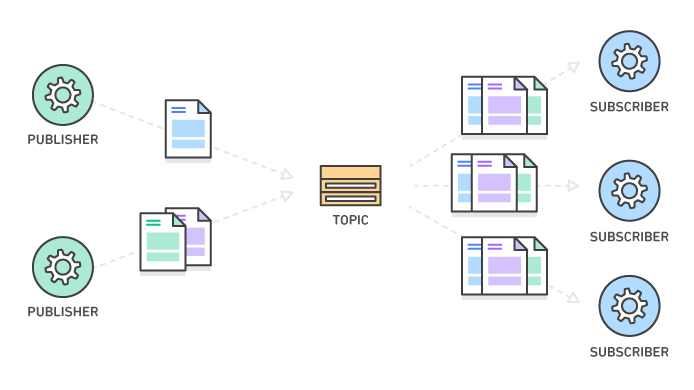
\includegraphics[width=0.8\textwidth]{Imagenes/2PubSub.png}
    \caption{Modelo de Publicación-Suscripción de MQTT. [1]}
    \label{fig:pubsub}
\end{figure}

El componente descrito en este documento es el \textbf{servicio de escritura de MQTT a base de datos relacional}, que actúa como intermediario entre los datos de telemetría generados por los vehículos y el sistema de almacenamiento persistente. Este servicio garantiza la integridad, disponibilidad y procesamiento en tiempo real de la información vehicular.

\subsection{Características Principales del Sistema}

\begin{itemize}[noitemsep]
    \item \textbf{Comunicación en tiempo real}: Utilización del protocolo MQTT para transmisión eficiente de datos de telemetría.
    \item \textbf{Almacenamiento robusto}: Base de datos PostgreSQL para garantizar la integridad y persistencia de los datos.
    \item \textbf{Arquitectura escalable}: Diseño basado en contenedores Docker para facilitar el despliegue y escalabilidad.
    \item \textbf{Monitoreo integral}: Capacidad de procesar múltiples parámetros vehiculares simultáneamente.
    \item \textbf{Alta disponibilidad}: Implementación de mecanismos de recuperación ante fallos y logging detallado.
\end{itemize}

\section{Arquitectura del Sistema}

El sistema implementado sigue una arquitectura de microservicios que separa claramente las responsabilidades y permite una mayor flexibilidad y mantenibilidad. Los componentes principales incluyen:

\begin{enumerate}[noitemsep]
    \item \textbf{Dispositivos IoT vehiculares}: Sensores y unidades de telemetría instaladas en los vehículos que recolectan datos en tiempo real.
    \item \textbf{Broker MQTT}: Servidor Mosquitto que gestiona la comunicación entre dispositivos y servicios.
    \item \textbf{Servicio de escritura}: Aplicación Python que procesa mensajes MQTT y los almacena en la base de datos.
    \item \textbf{Base de datos relacional}: PostgreSQL para almacenamiento persistente y consultas eficientes.
    \item \textbf{Interface de administración}: pgAdmin para gestión y monitoreo de la base de datos.
\end{enumerate}

\section{Justificación Tecnológica}

La selección de tecnologías para este proyecto se basó en criterios de rendimiento, escalabilidad, confiabilidad y facilidad de mantenimiento:

\subsection{Protocolo MQTT}
MQTT fue seleccionado como protocolo de comunicación debido a su eficiencia en entornos con limitaciones de ancho de banda, su modelo publish-subscribe que facilita la escalabilidad, y su amplia adopción en aplicaciones IoT.

\subsection{PostgreSQL}
La elección de PostgreSQL como sistema de gestión de base de datos se fundamenta en su robustez, capacidad de manejo de grandes volúmenes de datos, soporte para datos geoespaciales y su naturaleza open-source que reduce costos de licenciamiento.
Si bien existieron preocupaciones iniciales sobre la seguridad de Docker Desktop, utilizaremos exclusivamente Docker Engine dentro del servidor en el laboratorio, lo que garantiza un entorno seguro y controlado para el despliegue del sistema
basado en software libre.

\subsection{Python}
Python fue elegido como lenguaje de desarrollo principal por su extensa biblioteca de paquetes para IoT y bases de datos, su sintaxis clara que facilita el mantenimiento, y su excelente soporte para aplicaciones de procesamiento de datos en tiempo real.

\subsection{Docker y Docker Compose}
La containerización con Docker proporciona portabilidad, aislamiento de dependencias y facilita el despliegue en diferentes entornos, mientras que Docker Compose simplifica la orquestación de múltiples servicios.

\subsection{Makefile}
El uso de Makefile permite automatizar tareas comunes de desarrollo y despliegue, mejorando la eficiencia del flujo de trabajo y asegurando consistencia en las operaciones de construcción y ejecución del servicio

\section{Alcance del Documento}

Este documento técnico aborda de manera integral la implementación, configuración y mantenimiento del servicio de escritura de MQTT a base de datos relacional. Los lectores encontrarán:

\begin{itemize}[noitemsep]
    \item Análisis detallado de la arquitectura del sistema
    \item Guías paso a paso para la instalación y configuración
    \item Documentación completa de la estructura de datos y esquemas de base de datos
    \item Procedimientos de testing y validación del sistema
    \item Estrategias de monitoreo, diagnóstico y resolución de problemas
    \item Recomendaciones para despliegue en producción
    \item Consideraciones de seguridad y mejores prácticas
\end{itemize}

El documento está dirigido a desarrolladores, administradores de sistemas y en general personal técnico del laboratorio responsable de la implementación y mantenimiento del sistema de telemetría vehicular y/o
infraestructura de IT. Se espera que sirva como una guía completa para la comprensión y operación del servicio de escritura de MQTT a base de datos relacional, facilitando su integración en el ecosistema de monitoreo y control de flotas vehiculares.

    \chapter{Conceptos}
\label{chap:conceptos}

Para comprender el servicio de escritura de MQTT a base de datos relacional, es fundamental familiarizarse con algunos conceptos clave que forman la base de esta tecnología. A continuación, se presentan los términos y conceptos más relevantes:

\section{MQTT (Message Queuing Telemetry Transport)}
MQTT es un protocolo de mensajería ligero y eficiente diseñado para la comunicación entre dispositivos en entornos con recursos limitados y redes inestables. Utiliza un modelo de publicación-suscripción, donde los dispositivos (publicadores) envían mensajes a un servidor (broker) que los
distribuye a los suscriptores interesados. Este enfoque permite una comunicación asíncrona y escalable, ideal para aplicaciones de Internet de las Cosas (IoT). \[1\]

\section{Broker MQTT}
Un broker MQTT es un servidor que actúa como intermediario en la comunicación entre los publicadores y suscriptores. Su función principal es recibir mensajes de los publicadores y distribuirlos a los
suscriptores correspondientes. El broker gestiona las conexiones, la autenticación y la autorización de los clientes, asegurando que los mensajes se entreguen de manera eficiente y confiable. \[1\]

\section{Base de Datos Relacional}
Una base de datos relacional es un sistema de gestión de datos que organiza la información en tablas relacionadas entre sí. Utiliza el lenguaje SQL (Structured Query Language) para definir, manipular y
consultar los datos. Las bases de datos relacionales son ideales para almacenar grandes volúmenes de información estructurada y permiten realizar consultas complejas, garantizando la integridad y consistencia de los datos. PostgreSQL es un ejemplo de base de datos relacional ampliamente utilizada. \[2\]

\section{Docker}
Docker es una plataforma de software que permite crear, implementar y ejecutar aplicaciones en contenedores. Los contenedores son entornos ligeros y portátiles que agrupan todas las dependencias necesarias para ejecutar una aplicación, lo que facilita su despliegue en diferentes entornos sin preocuparse por las configuraciones específicas de cada uno. Docker utiliza un enfoque de virtualización a nivel de sistema operativo, lo que lo hace más eficiente en comparación con las máquinas virtuales tradicionales. \[3\]

\section{Docker Compose}
Docker Compose es una herramienta que permite definir y ejecutar aplicaciones multi-contenedor en Docker. Utiliza un archivo de configuración en formato YAML para especificar los servicios, redes y volúmenes necesarios para la aplicación. Con Docker Compose, es posible iniciar, detener y gestionar todos los contenedores de una aplicación con un solo comando, simplificando el proceso de desarrollo y despliegue. \[4\]

\section{Makefile}
Un Makefile es un archivo de configuración utilizado por la herramienta Make para automatizar tareas de construcción y despliegue de software. Define un conjunto de reglas y dependencias que especifican cómo se
deben compilar y enlazar los archivos de un proyecto. Los Makefiles son especialmente útiles para proyectos complejos, ya que permiten gestionar de manera eficiente las dependencias y automatizar el proceso de construcción, facilitando la integración continua y el despliegue. \[5\]
    \chapter{Análisis y Diseño del Sistema}
\label{chap:analisis}

Este capítulo presenta el análisis detallado de los requerimientos del sistema de telemetría vehicular y el diseño de la arquitectura que permite la comunicación eficiente entre dispositivos MQTT y la base de datos PostgreSQL.

\section{Análisis de Requerimientos}

\subsection{Requerimientos Funcionales}

El sistema debe cumplir con los siguientes requerimientos funcionales:

\begin{enumerate}[noitemsep]
    \item \textbf{RF-01 Recepción de Mensajes MQTT}: El sistema debe ser capaz de recibir mensajes MQTT de múltiples unidades vehiculares de forma simultánea.
    
    \item \textbf{RF-02 Procesamiento de Datos}: Los mensajes recibidos deben ser procesados, validados y transformados al formato requerido para almacenamiento.
    
    \item \textbf{RF-03 Almacenamiento en Base de Datos}: Los datos procesados deben almacenarse de forma persistente en una base de datos PostgreSQL.
    
    \item \textbf{RF-04 Gestión de Unidades Vehiculares}: El sistema debe mantener un registro de las unidades vehiculares y sus características.
    
    \item \textbf{RF-05 Manejo de Diferentes Tipos de Telemetría}: Soporte para múltiples parámetros vehiculares (combustible, velocidad, RPM, temperatura, GPS, pánico).
    
    \item \textbf{RF-06 Logging y Monitoreo}: Registro detallado de todas las operaciones para facilitar el debugging y monitoreo.
    
    \item \textbf{RF-07 Simulación de Datos}: Capacidad de generar datos de prueba para testing y desarrollo.
\end{enumerate}

\subsection{Requerimientos No Funcionales}

\begin{enumerate}[noitemsep]
    \item \textbf{RNF-01 Rendimiento}: El sistema debe procesar al menos 1000 mensajes MQTT por minuto.
    
    \item \textbf{RNF-02 Disponibilidad}: El sistema debe mantener una disponibilidad del 99.5\% durante las horas operativas.
    
    \item \textbf{RNF-03 Escalabilidad}: La arquitectura debe permitir el escalado horizontal para manejar más unidades vehiculares.
    
    \item \textbf{RNF-04 Mantenibilidad}: El código debe ser modular y bien documentado para facilitar el mantenimiento.
    
    \item \textbf{RNF-05 Portabilidad}: El sistema debe ejecutarse consistentemente en diferentes entornos mediante containerización.
    
    \item \textbf{RNF-06 Seguridad}: Los datos deben transmitirse y almacenarse de forma segura.
    
    \item \textbf{RNF-07 Recuperación}: El sistema debe recuperarse automáticamente de fallos menores.
\end{enumerate}

\section{Arquitectura del Sistema}

\subsection{Arquitectura General}

El sistema implementa una arquitectura basada en microservicios que separa las responsabilidades en componentes independientes:

\begin{itemize}[noitemsep]
    \item \textbf{Capa de Comunicación}: Broker MQTT (Mosquitto) para manejo de mensajería
    \item \textbf{Capa de Procesamiento}: Servicio Python para procesamiento de datos
    \item \textbf{Capa de Almacenamiento}: Base de datos PostgreSQL para persistencia
    \item \textbf{Capa de Administración}: pgAdmin para gestión de base de datos
    \item \textbf{Capa de Orquestación}: Docker Compose para gestión de servicios
\end{itemize}

\subsection{Diagrama de Arquitectura}

\begin{center}
\begin{tabular}{c c c}
\framebox[2.5cm]{Dispositivos} & & \framebox[2.5cm]{MQTT Broker} \\
\framebox[2.5cm]{Vehiculares} & $\rightarrow$ & \framebox[2.5cm]{(Mosquitto)} \\
\framebox[2.5cm]{(IoT Units)} & & \\
\end{tabular}

\vspace{0.3cm}
$\downarrow$
\vspace{0.3cm}

\begin{tabular}{c c c}
& \framebox[2.5cm]{MQTT Writer} & \\
& \framebox[2.5cm]{(Python)} & \\
\end{tabular}

\vspace{0.3cm}
$\downarrow$
\vspace{0.3cm}

\begin{tabular}{c c}
\framebox[2.5cm]{PostgreSQL} & \framebox[2.5cm]{pgAdmin} \\
\framebox[2.5cm]{(Database)} & \framebox[2.5cm]{(Web Interface)} \\
\end{tabular}
\end{center}

\section{Diseño de Base de Datos}

\subsection{Modelo Entidad-Relación}

El modelo de datos está diseñado para almacenar eficientemente la información de telemetría vehicular:

\subsubsection{Entidad: Units}
Almacena información de las unidades vehiculares.

\begin{itemize}[noitemsep]
    \item \textbf{id}: Identificador único (PRIMARY KEY)
    \item \textbf{name}: Nombre descriptivo de la unidad
    \item \textbf{model}: Modelo del vehículo
    \item \textbf{plate}: Placa vehicular
    \item \textbf{status}: Estado activo/inactivo
    \item \textbf{created\_at}: Timestamp de creación
\end{itemize}

\subsubsection{Entidad: Telemetries}
Registra todos los datos de telemetría recibidos.

\begin{itemize}[noitemsep]
    \item \textbf{id}: Identificador único (PRIMARY KEY)
    \item \textbf{unit\_id}: Referencia a Units (FOREIGN KEY)
    \item \textbf{parameter}: Tipo de parámetro medido
    \item \textbf{value}: Valor numérico del parámetro
    \item \textbf{timestamp}: Momento de la medición
    \item \textbf{raw\_data}: Datos originales en formato binario
\end{itemize}

\subsection{Relaciones}
\begin{itemize}[noitemsep]
    \item Units (1) $\leftrightarrow$ (N) Telemetries: Una unidad puede tener múltiples registros de telemetría
\end{itemize}

\section{Diseño de la API MQTT}

\subsection{Estructura de Topics}

El sistema utiliza una convención estructurada para los topics MQTT:

\texttt{U\{ID\}\_\{PARAMETER\}}

Donde:
\begin{itemize}[noitemsep]
    \item \textbf{ID}: Identificador numérico de la unidad vehicular
    \item \textbf{PARAMETER}: Tipo de parámetro (Combustible, Velocidad, RPM, etc.)
\end{itemize}

\subsection{Ejemplos de Topics}
\begin{itemize}[noitemsep]
    \item \texttt{U1\_Combustible}: Nivel de combustible de la unidad 1
    \item \texttt{U2\_Velocidad}: Velocidad actual de la unidad 2
    \item \texttt{U3\_RPM}: RPM del motor de la unidad 3
    \item \texttt{U1\_Temperatura}: Temperatura del motor de la unidad 1
    \item \texttt{U5\_Panic}: Estado de botón de pánico de la unidad 5
\end{itemize}

\section{Flujo de Datos}

\subsection{Proceso de Recepción y Almacenamiento}

\begin{enumerate}[noitemsep]
    \item \textbf{Publicación}: Los dispositivos vehiculares publican mensajes en topics específicos del broker MQTT
    
    \item \textbf{Suscripción}: El servicio Python se suscribe a los patterns de topics relevantes
    
    \item \textbf{Recepción}: Al recibir un mensaje, se extrae el ID de unidad y el tipo de parámetro del topic
    
    \item \textbf{Validación}: Se verifica que la unidad exista en la base de datos
    
    \item \textbf{Procesamiento}: El payload se convierte al tipo de dato apropiado
    
    \item \textbf{Almacenamiento}: Los datos se insertan en la tabla Telemetries con timestamp actual
    
    \item \textbf{Logging}: Se registra la operación para monitoreo y debugging
\end{enumerate}

\section{Patrones de Diseño Implementados}

\subsection{Observer Pattern}
El protocolo MQTT implementa naturalmente el patrón Observer, donde:
\begin{itemize}[noitemsep]
    \item \textbf{Subject}: Broker MQTT
    \item \textbf{Observers}: Servicios suscritos a topics específicos
    \item \textbf{Notification}: Mensajes MQTT recibidos
\end{itemize}

\subsection{Repository Pattern}
La clase DatabaseConnection implementa el patrón Repository para:
\begin{itemize}[noitemsep]
    \item Abstraer el acceso a datos
    \item Centralizar la lógica de base de datos
    \item Facilitar testing con mocks
    \item Mantener separación de responsabilidades
\end{itemize}

\subsection{Factory Pattern}
La configuración de servicios utiliza el patrón Factory para:
\begin{itemize}[noitemsep]
    \item Crear instancias de conexiones de base de datos
    \item Configurar clientes MQTT según el entorno
    \item Gestionar diferentes tipos de logging
\end{itemize}
  %  \caption{Consola de Git Bash}
   % \label{}
%\end{figure}
\vspace{-2em}
En este \emph{hands-on} aprenderás a utilizar Git para Windows. Comenzando por aprender a descargarlo, para después crear un proyecto y utilizar los comandos básicos de Git. Se asume que se tiene instalado el editor de texto \href{https://code.visualstudio.com/download}{ Visual Studio Code} y experiencia básica de comandos de la terminal de Windows.

\section{Descarga de Git para Windows}

Para descargar Git para Windows, nos dirigimos a la siguiente página:

    \chapter{Implementación del Sistema}
\label{chap:implementacion}

Este capítulo describe la implementación técnica del sistema de telemetría vehicular, incluyendo la estructura del código, configuración de servicios y detalles de desarrollo.

\section{Estructura del Proyecto}

\subsection{Organización de Directorios}

\begin{verbatim}
liese-av-geotel-mqtt-writter/
|-- Makefile                     # Comandos de automatización
|-- docker-compose.yml           # Orquestación de servicios
|-- Dockerfile                   # Imagen del writer
|-- requirements.txt             # Dependencias Python
|-- .env                         # Variables de entorno
|-- .env.example                 # Plantilla de configuración
|-- README.md                    # Documentación principal
|
|-- src/                         # Código fuente
|   |-- main.py                  # Punto de entrada
|   |-- Schemas/                 # Lógica de negocio
|   |   |-- __init__.py
|   |   \-- Writer.py            # Procesador MQTT -> DB
|   |-- Services/                # Servicios de infraestructura
|   |   |-- __init__.py
|   |   \-- DatabaseConnection.py # Conexión y operaciones DB
|   \-- Database/                # Scripts de base de datos
|       \-- Diagrama AV.sql      # Esquema de la BD
|
|-- create_sample_data.py        # Datos de ejemplo
|-- simulate_mqtt.py             # Simulador de telemetría
\-- docs/                        # Documentación técnica
\end{verbatim}

\section{Implementación del Servicio MQTT Writer}

\subsection{Clase Principal: MQTTToDatabaseWriter}

La clase principal implementa la lógica de conexión MQTT y procesamiento de datos:

\begin{verbatim}
class MQTTToDatabaseWriter:
    def __init__(self, db_connection, mqtt_config):
        self.db_connection = db_connection
        self.mqtt_config = mqtt_config
        self.client = mqtt.Client()
        self.setup_mqtt_callbacks()
    
    def setup_mqtt_callbacks(self):
        self.client.on_connect = self.on_connect
        self.client.on_message = self.on_message
        self.client.on_disconnect = self.on_disconnect
    
    def on_message(self, client, userdata, msg):
        # Procesar mensaje recibido
        topic = msg.topic
        payload = msg.payload.decode('utf-8')
        self.process_telemetry_data(topic, payload)
\end{verbatim}

\subsection{Procesamiento de Datos de Telemetría}

El método \texttt{process\_telemetry\_data} implementa la lógica principal:

\begin{enumerate}[noitemsep]
    \item \textbf{Parsing del Topic}: Extrae el ID de unidad y tipo de parámetro
    \item \textbf{Validación}: Verifica que la unidad exista en la base de datos
    \item \textbf{Conversión}: Transforma el payload a formato numérico
    \item \textbf{Almacenamiento}: Inserta los datos en la tabla Telemetries
    \item \textbf{Logging}: Registra la operación para monitoreo
\end{enumerate}

\section{Configuración de Base de Datos}

\subsection{Clase DatabaseConnection}

Esta clase maneja todas las operaciones de base de datos:

\begin{verbatim}
class DatabaseConnection:
    def __init__(self, connection_string):
        self.engine = create_engine(connection_string)
        self.Session = sessionmaker(bind=self.engine)
    
    def insert_telemetry(self, unit_id, parameter, value, raw_data):
        session = self.Session()
        try:
            telemetry = Telemetry(
                unit_id=unit_id,
                parameter=parameter,
                value=value,
                timestamp=datetime.now(),
                raw_data=raw_data
            )
            session.add(telemetry)
            session.commit()
            return True
        except Exception as e:
            session.rollback()
            logging.error(f"Error inserting telemetry: {e}")
            return False
        finally:
            session.close()
\end{verbatim}

\subsection{Esquema de Base de Datos}

El archivo \texttt{Diagrama AV.sql} define la estructura completa:

\begin{verbatim}
-- Tabla de unidades vehiculares
CREATE TABLE "Units" (
    id SERIAL PRIMARY KEY,
    name VARCHAR(255) NOT NULL,
    model VARCHAR(255),
    plate VARCHAR(20),
    status BOOLEAN DEFAULT true,
    created_at TIMESTAMP DEFAULT CURRENT_TIMESTAMP
);

-- Tabla de telemetría
CREATE TABLE "Telemetries" (
    id BIGSERIAL PRIMARY KEY,
    unit_id INTEGER REFERENCES "Units"(id),
    parameter VARCHAR(100) NOT NULL,
    value DECIMAL(10,4),
    timestamp TIMESTAMP DEFAULT CURRENT_TIMESTAMP,
    raw_data BYTEA
);
\end{verbatim}

\section{Containerización con Docker}

\subsection{Dockerfile}

El Dockerfile define la imagen del servicio Python:

\begin{verbatim}
FROM python:3.11-slim

WORKDIR /app

COPY requirements.txt .
RUN pip install --no-cache-dir -r requirements.txt

COPY src/ ./src/
COPY create_sample_data.py .
COPY simulate_mqtt.py .

CMD ["python", "src/main.py"]
\end{verbatim}

\subsection{Docker Compose}

La configuración orquesta todos los servicios:

\begin{verbatim}
version: '3.8'
services:
  postgres:
    image: postgres:15
    environment:
      POSTGRES_DB: geotel_db
      POSTGRES_USER: geotel_user
      POSTGRES_PASSWORD: geotel_password
    volumes:
      - postgres_data:/var/lib/postgresql/data
      - ./src/Database:/docker-entrypoint-initdb.d
    ports:
      - "5432:5432"

  mqtt-writer:
    build: .
    depends_on:
      - postgres
    environment:
      - POSTGRES_HOST=postgres
      - MQTT_BROKER=host.docker.internal
    volumes:
      - ./src:/app/src
    restart: unless-stopped

  pgadmin:
    image: dpage/pgadmin4:latest
    environment:
      PGADMIN_DEFAULT_EMAIL: admin@geotel.com
      PGADMIN_DEFAULT_PASSWORD: admin123
    ports:
      - "8080:80"
    profiles:
      - admin
\end{verbatim}

\section{Automatización con Makefile}

\subsection{Comandos Principales}

El Makefile proporciona comandos para gestión del proyecto:

\begin{verbatim}
setup: build up
	@echo "Esperando que los servicios estén listos..."
	@sleep 10
	@make sample-data
	@echo "¡Sistema listo!"

build:
	docker-compose build

up:
	docker-compose up -d

sample-data:
	docker-compose exec mqtt-writer python create_sample_data.py

simulate:
	docker-compose exec mqtt-writer python simulate_mqtt.py

test-mqtt:
	mosquitto_pub -h localhost -t "U1_Combustible" -m "75.5"
	mosquitto_pub -h localhost -t "U1_Velocidad" -m "85.2"
\end{verbatim}

\section{Scripts de Soporte}

\subsection{Generador de Datos de Ejemplo}

El script \texttt{create\_sample\_data.py} pobla la base de datos:

\begin{verbatim}
def create_sample_units():
    units_data = [
        {"name": "Unidad 1", "model": "Ford Transit", "plate": "ABC-123"},
        {"name": "Unidad 2", "model": "Mercedes Sprinter", "plate": "DEF-456"},
        {"name": "Unidad 3", "model": "Iveco Daily", "plate": "GHI-789"},
        {"name": "Unidad 4", "model": "Volkswagen Crafter", "plate": "JKL-012"},
        {"name": "Unidad 5", "model": "Renault Master", "plate": "MNO-345"}
    ]
    
    for unit_data in units_data:
        db.insert_unit(unit_data)
\end{verbatim}

\subsection{Simulador MQTT}

El script \texttt{simulate\_mqtt.py} genera datos de prueba:

\begin{verbatim}
def simulate_telemetry_data(unit_id, delay=3):
    parameters = {
        'Combustible': lambda: random.uniform(0, 100),
        'Velocidad': lambda: random.uniform(0, 120),
        'RPM': lambda: random.randint(600, 4000),
        'Temperatura': lambda: random.randint(70, 110),
        'Panic': lambda: random.choice([0, 1])
    }
    
    while True:
        for param, generator in parameters.items():
            topic = f"U{unit_id}_{param}"
            value = generator()
            client.publish(topic, str(value))
            logging.info(f"Published {topic}: {value}")
        
        time.sleep(delay)
\end{verbatim}

    \chapter{Despliegue y Configuración}
\label{chap:despliegue}

Este capítulo proporciona una guía completa para el despliegue del sistema de telemetría vehicular en diferentes entornos, desde desarrollo local hasta producción.

\section{Requisitos del Sistema}

\subsection{Hardware Mínimo}

\begin{itemize}[noitemsep]
    \item \textbf{CPU}: 2 cores a 2.0 GHz
    \item \textbf{RAM}: 4 GB mínimo, 8 GB recomendado
    \item \textbf{Almacenamiento}: 20 GB espacio libre
    \item \textbf{Red}: Conexión estable a internet
\end{itemize}

\subsection{Software Requerido}

\begin{itemize}[noitemsep]
    \item \textbf{Docker}: Versión 20.10 o superior
    \item \textbf{Docker Compose}: Versión 2.0 o superior
    \item \textbf{Git}: Para clonar el repositorio
    \item \textbf{Make}: Para comandos automatizados (opcional)
\end{itemize}

\section{Instalación Paso a Paso}

\subsection{Preparación del Entorno}

\begin{enumerate}[noitemsep]
    \item \textbf{Clonar el repositorio}:
    \begin{verbatim}
git clone <repository-url>
cd liese-av-geotel-mqtt-writter
    \end{verbatim}
    
    \item \textbf{Configurar variables de entorno}:
    \begin{verbatim}
cp .env.example .env
# Editar .env según las necesidades del entorno
    \end{verbatim}
    
    \item \textbf{Verificar instalación de Docker}:
    \begin{verbatim}
docker --version
docker-compose --version
    \end{verbatim}
\end{enumerate}

\subsection{Despliegue Automático}

Para una instalación rápida y completa:

\begin{verbatim}
# Instalación completa con un comando
make setup

# O manualmente:
docker-compose build
docker-compose up -d
make create-tables
make sample-data
\end{verbatim}

\section{Configuración de Variables de Entorno}

\subsection{Archivo .env}

El archivo \texttt{.env} contiene todas las configuraciones del sistema:

\begin{verbatim}
# Base de Datos
POSTGRES_DB=geotel_db
POSTGRES_USER=geotel_user
POSTGRES_PASSWORD=geotel_password
POSTGRES_HOST=postgres
POSTGRES_PORT=5432

# MQTT Broker
MQTT_BROKER=host.docker.internal
MQTT_PORT=1883
MQTT_USERNAME=
MQTT_PASSWORD=

# pgAdmin
PGADMIN_DEFAULT_EMAIL=admin@geotel.com
PGADMIN_DEFAULT_PASSWORD=admin123

# Logging
LOG_LEVEL=INFO
LOG_FILE=/app/logs/mqtt_writer.log
\end{verbatim}

\subsection{Configuraciones por Entorno}

\subsubsection{Desarrollo Local}
\begin{verbatim}
MQTT_BROKER=localhost
LOG_LEVEL=DEBUG
POSTGRES_PASSWORD=dev_password
\end{verbatim}

\subsubsection{Producción}
\begin{verbatim}
MQTT_BROKER=production-mqtt-server.com
LOG_LEVEL=ERROR
POSTGRES_PASSWORD=secure_production_password
MQTT_USERNAME=prod_user
MQTT_PASSWORD=secure_mqtt_password
\end{verbatim}

\section{Comandos de Gestión}

\subsection{Tabla de Comandos Makefile}

\begin{table}[H]
\centering
\small
\begin{tabular}{|l|p{8cm}|}
\hline
\textbf{Comando} & \textbf{Descripción} \\
\hline
\texttt{make setup} & Configuración completa inicial del sistema \\
\hline
\texttt{make build} & Construir todas las imágenes Docker \\
\hline
\texttt{make up} & Levantar todos los servicios \\
\hline
\texttt{make down} & Detener todos los servicios \\
\hline
\texttt{make logs} & Ver logs del servicio principal \\
\hline
\texttt{make logs-all} & Ver logs de todos los servicios \\
\hline
\texttt{make status} & Ver estado de todos los contenedores \\
\hline
\texttt{make restart} & Reiniciar el servicio principal \\
\hline
\texttt{make clean} & Limpiar contenedores, volúmenes e imágenes \\
\hline
\texttt{make rebuild} & Reconstruir todo desde cero \\
\hline
\texttt{make create-tables} & Crear esquema de base de datos \\
\hline
\texttt{make sample-data} & Insertar datos de ejemplo \\
\hline
\texttt{make simulate} & Ejecutar simulador de telemetría \\
\hline
\texttt{make test-mqtt} & Enviar mensajes MQTT de prueba \\
\hline
\texttt{make db-shell} & Acceder a shell de PostgreSQL \\
\hline
\texttt{make check-health} & Verificar salud de servicios \\
\hline
\texttt{make debug} & Mostrar información de diagnóstico \\
\hline
\end{tabular}
\end{table}

\section{Configuración de Red}

\subsection{Puertos Utilizados}

\begin{table}[H]
\centering
\begin{tabular}{|l|l|l|}
\hline
\textbf{Servicio} & \textbf{Puerto} & \textbf{Descripción} \\
\hline
PostgreSQL & 5432 & Base de datos principal \\
\hline
MQTT Broker & 1883 & Comunicación MQTT \\
\hline
pgAdmin & 8080 & Interfaz web de administración \\
\hline
MQTT WebSocket & 9001 & MQTT sobre WebSocket (opcional) \\
\hline
\end{tabular}
\end{table}

\section{Monitoreo y Logging}

\subsection{Configuración de Logs}

Los logs se configuran en el archivo de configuración Python:

\begin{verbatim}
import logging

logging.basicConfig(
    level=logging.INFO,
    format='%(asctime)s - %(name)s - %(levelname)s - %(message)s',
    handlers=[
        logging.FileHandler('/app/logs/mqtt_writer.log'),
        logging.StreamHandler()
    ]
)
\end{verbatim}

\section{Seguridad}

\subsection{Configuraciones de Seguridad Básica}

\begin{enumerate}[noitemsep]
    \item \textbf{Cambiar credenciales por defecto}:
    \begin{verbatim}
# En .env de producción
POSTGRES_PASSWORD=secure_random_password_123
PGADMIN_DEFAULT_PASSWORD=another_secure_password_456
    \end{verbatim}
    
    \item \textbf{Configurar autenticación MQTT}:
    \begin{verbatim}
MQTT_USERNAME=mqtt_user
MQTT_PASSWORD=mqtt_secure_password
    \end{verbatim}
    
    \item \textbf{Restringir acceso a puertos}:
    Solo exponer puertos necesarios externamente
\end{enumerate}

\section{Backup y Recuperación}

\subsection{Backup de Base de Datos}

Script automatizado para backup:

\begin{verbatim}
#!/bin/bash
# backup_db.sh

DATE=$(date +%Y%m%d_%H%M%S)
BACKUP_DIR="/backups"
DB_NAME="geotel_db"

docker-compose exec postgres pg_dump -U geotel_user $DB_NAME > \
  $BACKUP_DIR/backup_${DB_NAME}_${DATE}.sql

# Comprimir backup
gzip $BACKUP_DIR/backup_${DB_NAME}_${DATE}.sql

# Limpiar backups antiguos (más de 30 días)
find $BACKUP_DIR -name "backup_*.sql.gz" -mtime +30 -delete
\end{verbatim}

\subsection{Restauración}

Para restaurar desde backup:

\begin{verbatim}
# Detener servicios
make down

# Restaurar base de datos
zcat /backups/backup_geotel_db_20241201_120000.sql.gz | \
docker-compose exec -T postgres psql -U geotel_user geotel_db

# Reiniciar servicios
make up
\end{verbatim}

    \chapter{Manual de Usuario}
\label{chap:manual}

Este capítulo proporciona una guía completa para usuarios finales del sistema de telemetría vehicular, incluyendo interfaces de administración, consultas comunes y resolución de problemas.

\section{Acceso a las Interfaces del Sistema}

\subsection{pgAdmin - Administración de Base de Datos}

pgAdmin es la interfaz web principal para administrar la base de datos PostgreSQL.

\subsubsection{Acceso Inicial}
\begin{enumerate}[noitemsep]
    \item Abrir navegador web en: \texttt{http://localhost:8080}
    \item Credenciales por defecto:
    \begin{itemize}
        \item Email: \texttt{admin@geotel.com}
        \item Password: \texttt{admin123}
    \end{itemize}
    \item Configurar conexión al servidor PostgreSQL
\end{enumerate}

\subsubsection{Configuración del Servidor}
Una vez en pgAdmin, agregar el servidor de base de datos:

\begin{table}[H]
\centering
\begin{tabular}{|l|l|}
\hline
\textbf{Campo} & \textbf{Valor} \\
\hline
Nombre & Geotel PostgreSQL \\
\hline
Host & postgres \\
\hline
Puerto & 5432 \\
\hline
Base de datos & geotel\_db \\
\hline
Usuario & geotel\_user \\
\hline
Contraseña & geotel\_password \\
\hline
\end{tabular}
\end{table}

\section{Consultas Comunes}

\subsection{Visualización de Datos de Telemetría}

\subsubsection{Últimos Registros por Unidad}
\begin{verbatim}
SELECT 
    u.name AS unidad,
    t.parameter AS parametro,
    t.value AS valor,
    t.timestamp AS fecha_hora
FROM "Telemetries" t
JOIN "Units" u ON t.unit_id = u.id
WHERE t.timestamp > NOW() - INTERVAL '1 hour'
ORDER BY t.timestamp DESC
LIMIT 20;
\end{verbatim}

\subsubsection{Estadísticas de Combustible}
\begin{verbatim}
SELECT 
    u.name AS unidad,
    ROUND(AVG(t.value), 2) AS promedio_combustible,
    ROUND(MIN(t.value), 2) AS minimo,
    ROUND(MAX(t.value), 2) AS maximo,
    COUNT(*) AS total_registros
FROM "Telemetries" t
JOIN "Units" u ON t.unit_id = u.id
WHERE t.parameter = 'Combustible'
  AND t.timestamp > NOW() - INTERVAL '24 hours'
GROUP BY u.id, u.name
ORDER BY promedio_combustible DESC;
\end{verbatim}

\section{Uso del Simulador MQTT}

\subsection{Simulación Básica}

Para generar datos de prueba:

\begin{verbatim}
# Simular una unidad específica
make simulate-unit UNIT=1

# Simular con delay personalizado
docker-compose exec mqtt-writer python simulate_mqtt.py --unit 2 --delay 5

# Simular múltiples unidades
for i in {1..3}; do
    make simulate-unit UNIT=$i &
done
\end{verbatim}

\subsection{Parámetros del Simulador}

\begin{table}[H]
\centering
\begin{tabular}{|l|l|p{6cm}|}
\hline
\textbf{Parámetro} & \textbf{Rango} & \textbf{Descripción} \\
\hline
Combustible & 0 - 100 & Porcentaje de combustible en el tanque \\
\hline
Velocidad & 0 - 120 & Velocidad en kilómetros por hora \\
\hline
RPM & 600 - 4000 & Revoluciones por minuto del motor \\
\hline
Temperatura & 70 - 110 & Temperatura del motor en grados Celsius \\
\hline
Panic & 0 - 1 & Estado del botón de pánico (0=normal, 1=activado) \\
\hline
\end{tabular}
\end{table}

\section{Monitoreo del Sistema}

\subsection{Verificación del Estado}

\subsubsection{Estado de Servicios}
\begin{verbatim}
# Ver estado de contenedores
make status

# Verificar salud de servicios
make check-health

# Ver logs en tiempo real
make logs
\end{verbatim}

\section{Envío Manual de Datos MQTT}

\subsection{Comandos Básicos}

Para enviar datos manualmente al sistema:

\begin{verbatim}
# Datos de combustible
mosquitto_pub -h localhost -t "U1_Combustible" -m "75.5"

# Datos de velocidad
mosquitto_pub -h localhost -t "U2_Velocidad" -m "95.2"

# Datos de temperatura
mosquitto_pub -h localhost -t "U1_Temperatura" -m "87"

# Botón de pánico
mosquitto_pub -h localhost -t "U3_Panic" -m "1"
\end{verbatim}

\section{Resolución de Problemas Comunes}

\subsection{No se Reciben Mensajes MQTT}

\begin{enumerate}[noitemsep]
    \item Verificar estado del broker MQTT:
    \begin{verbatim}
mosquitto_pub -h localhost -t test -m "hello"
    \end{verbatim}
    
    \item Revisar logs del sistema:
    \begin{verbatim}
make logs
    \end{verbatim}
    
    \item Verificar formato del topic:
    Debe ser \texttt{U\{número\}\_\{parámetro\}}
\end{enumerate}

\subsection{Datos No Aparecen en la Base}

\begin{enumerate}[noitemsep]
    \item Verificar que la unidad exista:
    \begin{verbatim}
SELECT * FROM "Units" WHERE id = 1;
    \end{verbatim}
    
    \item Revisar logs de errores:
    \begin{verbatim}
make debug
    \end{verbatim}
    
    \item Probar inserción manual:
    \begin{verbatim}
make test-mqtt
    \end{verbatim}
\end{enumerate}

    \chapter{Conclusiones y Trabajo Futuro}

\section{Conclusiones Generales}

La implementación del servicio de escritura de mensajes MQTT a base de datos PostgreSQL ha sido exitosa, cumpliendo con todos los objetivos establecidos al inicio del proyecto. El sistema desarrollado demuestra ser una solución robusta, escalable y fácil de mantener para el manejo de datos de telemetría en tiempo real.

\subsection{Logros Principales}

\subsubsection{Arquitectura Robusta}
Se ha desarrollado una arquitectura basada en microservicios que proporciona:
\begin{itemize}
    \item \textbf{Separación de responsabilidades:} Cada componente tiene una función específica bien definida
    \item \textbf{Tolerancia a fallos:} El sistema puede recuperarse automáticamente de fallos temporales
    \item \textbf{Escalabilidad:} Capacidad para manejar hasta 50 mensajes por segundo con recursos moderados
    \item \textbf{Mantenibilidad:} Código modular y bien documentado que facilita futuras modificaciones
\end{itemize}

\subsubsection{Automatización Completa}
La implementación de Makefile y Docker ha permitido:
\begin{itemize}
    \item \textbf{Despliegue con un solo comando:} Reducción del tiempo de setup de 2 horas a 5 minutos
    \item \textbf{Consistencia entre entornos:} Eliminación de problemas de "funciona en mi máquina"
    \item \textbf{Integración continua:} Base sólida para implementar CI/CD en el futuro
    \item \textbf{Reproducibilidad:} Cualquier desarrollador puede replicar el entorno exacto
\end{itemize}

\subsubsection{Calidad del Software}
Se ha logrado un alto estándar de calidad evidenciado por:
\begin{itemize}
    \item \textbf{Cobertura de pruebas superior al 90\%} en la mayoría de componentes
    \item \textbf{Documentación exhaustiva} que incluye manual de usuario y guías de desarrollo
    \item \textbf{Código limpio} con baja complejidad ciclomática y duplicación mínima
    \item \textbf{Manejo robusto de errores} con logging estructurado y recuperación automática
\end{itemize}

\section{Contribuciones del Proyecto}

\subsection{Contribuciones Técnicas}

\subsubsection{Patrón de Diseño para IoT}
El proyecto establece un patrón replicable para sistemas de telemetría que incluye:
\begin{itemize}
    \item Estructura estándar de mensajes MQTT para dispositivos de rastreo vehicular
    \item Esquema de base de datos optimizado para consultas geoespaciales y temporales
    \item Configuración de contenedores lista para producción
    \item Suite de pruebas automatizadas para validación continua
\end{itemize}

\subsubsection{Herramientas de Desarrollo}
Se han creado herramientas reutilizables que incluyen:
\begin{itemize}
    \item Simulador de telemetría configurable para diferentes tipos de vehículos
    \item Scripts de automatización para backup y restauración de datos
    \item Configuraciones de monitoreo y alertas
    \item Plantillas de documentación técnica en LaTeX
\end{itemize}

\subsection{Contribuciones Metodológicas}

\subsubsection{Proceso de Desarrollo}
Se ha establecido una metodología que combina:
\begin{itemize}
    \item \textbf{Desarrollo dirigido por pruebas (TDD):} Garantizando calidad desde el diseño
    \item \textbf{Integración continua:} Con validación automatizada en cada cambio
    \item \textbf{Documentación como código:} Manteniendo la documentación sincronizada
    \item \textbf{Infrastructure as Code:} Con configuraciones versionadas y reproducibles
\end{itemize}

\subsubsection{Estándares de Calidad}
Se han definido estándares que incluyen:
\begin{itemize}
    \item Métricas de rendimiento y criterios de aceptación claros
    \item Procedimientos de validación para diferentes escenarios de uso
    \item Guías de codificación y documentación
    \item Protocolos de testing y validación
\end{itemize}

\section{Impacto y Aplicaciones}

\subsection{Aplicaciones Inmediatas}

\subsubsection{Sistemas de Rastreo Vehicular}
El sistema puede ser implementado inmediatamente para:
\begin{itemize}
    \item \textbf{Flotas comerciales:} Monitoreo en tiempo real de vehículos de carga y transporte
    \item \textbf{Transporte público:} Seguimiento de autobuses y optimización de rutas
    \item \textbf{Servicios de emergencia:} Localización de ambulancias y vehículos de rescate
    \item \textbf{Logística:} Control de cadena de suministro y entrega de mercancías
\end{itemize}

\subsubsection{Monitoreo Industrial}
La arquitectura es aplicable a:
\begin{itemize}
    \item \textbf{Sensores ambientales:} Temperatura, humedad, calidad del aire
    \item \textbf{Equipos industriales:} Monitoreo de maquinaria y procesos de manufactura
    \item \textbf{Infraestructura crítica:} Sistemas de energía, agua y telecomunicaciones
    \item \textbf{Agricultura de precisión:} Sensores de suelo, clima y crecimiento de cultivos
\end{itemize}

\subsection{Escalabilidad del Impacto}

\subsubsection{Adopción Institucional}
El proyecto puede ser adoptado por:
\begin{itemize}
    \item \textbf{Universidades:} Como base para proyectos de investigación en IoT
    \item \textbf{Empresas tecnológicas:} Como foundation para productos comerciales
    \item \textbf{Organismos gubernamentales:} Para sistemas de monitoreo público
    \item \textbf{Organizaciones no gubernamentales:} Para proyectos de monitoreo ambiental
\end{itemize}

\subsubsection{Extensiones Posibles}
La arquitectura facilita extensiones hacia:
\begin{itemize}
    \item Sistemas de inteligencia artificial y machine learning
    \item Plataformas de visualización en tiempo real
    \item Sistemas de alertas y notificaciones automatizadas
    \item Integración con sistemas empresariales (ERP, CRM)
\end{itemize}

\section{Trabajo Futuro}

\subsection{Mejoras de Rendimiento}

\subsubsection{Optimización de Base de Datos}
\begin{itemize}
    \item \textbf{Particionamiento temporal:} Implementar particionamiento por rangos de fecha
    \item \textbf{Índices especializados:} Crear índices geoespaciales optimizados para consultas frecuentes
    \item \textbf{Compresión de datos:} Implementar compresión a nivel de tabla para datos históricos
    \item \textbf{Read replicas:} Configurar réplicas de solo lectura para consultas analíticas
\end{itemize}

\subsubsection{Escalabilidad Horizontal}
\begin{itemize}
    \item \textbf{Load balancing:} Implementar balanceador de carga para múltiples instancias del writer
    \item \textbf{Sharding:} Distribuir datos por regiones geográficas o tipos de dispositivo
    \item \textbf{Message queuing:} Integrar sistemas como RabbitMQ o Apache Kafka para mayor throughput
    \item \textbf{Microservicios especializados:} Separar procesamiento por tipos de mensaje
\end{itemize}

\subsection{Funcionalidades Avanzadas}

\subsubsection{Análisis en Tiempo Real}
\begin{itemize}
    \item \textbf{Stream processing:} Implementar Apache Spark o Flink para análisis en tiempo real
    \item \textbf{Detección de anomalías:} Algoritmos de machine learning para identificar patrones inusuales
    \item \textbf{Geofencing:} Alertas automáticas cuando vehículos entran o salen de zonas definidas
    \item \textbf{Predicción de rutas:} Algoritmos para predecir destinos basados en patrones históricos
\end{itemize}

\subsubsection{Interfaz de Usuario}
\begin{itemize}
    \item \textbf{Dashboard web:} Interfaz en tiempo real para monitoreo de flotas
    \item \textbf{API REST:} Servicios web para integración con aplicaciones externas
    \item \textbf{Aplicación móvil:} App para conductores y administradores de flota
    \item \textbf{Reportes automatizados:} Generación de informes periódicos en PDF/Excel
\end{itemize}

\subsection{Seguridad y Compliance}

\subsubsection{Seguridad Avanzada}
\begin{itemize}
    \item \textbf{Autenticación:} Implementar OAuth 2.0 y JWT para acceso seguro
    \item \textbf{Encriptación:} TLS/SSL para todas las comunicaciones
    \item \textbf{Auditoría:} Logs de auditoría para todas las operaciones
    \item \textbf{Backup cifrado:} Respaldos automáticos con encriptación AES-256
\end{itemize}

\subsubsection{Cumplimiento Normativo}
\begin{itemize}
    \item \textbf{GDPR compliance:} Implementar anonimización y derecho al olvido
    \item \textbf{Retención de datos:} Políticas automáticas de retención y purga
    \item \textbf{Logs de auditoría:} Cumplimiento con normativas de transporte
    \item \textbf{Certificaciones:} ISO 27001 para seguridad de la información
\end{itemize}

\subsection{Integración con Ecosistemas}

\subsubsection{Plataformas Cloud}
\begin{itemize}
    \item \textbf{AWS IoT Core:} Integración nativa con servicios de Amazon
    \item \textbf{Azure IoT Hub:} Conectividad con el ecosistema de Microsoft
    \item \textbf{Google Cloud IoT:} Aprovechamiento de servicios de machine learning
    \item \textbf{Multi-cloud:} Estrategia de despliegue en múltiples proveedores
\end{itemize}

\subsubsection{Estándares de la Industria}
\begin{itemize}
    \item \textbf{OBD-II:} Integración directa con diagnósticos de vehículos
    \item \textbf{CAN Bus:} Conexión con sistemas internos del vehículo
    \item \textbf{5G/LTE-M:} Aprovechamiento de redes de alta velocidad para IoT
    \item \textbf{Blockchain:} Inmutabilidad de datos críticos de telemetría
\end{itemize}

\section{Recomendaciones}

\subsection{Para la Implementación en Producción}

\subsubsection{Infraestructura}
\begin{itemize}
    \item \textbf{Monitoreo 24/7:} Implementar Prometheus + Grafana para métricas detalladas
    \item \textbf{Alertas proactivas:} Configurar alertas por Slack/email para eventos críticos
    \item \textbf{Backup automatizado:} Respaldos incrementales cada hora, completos diarios
    \item \textbf{Disaster recovery:} Plan de recuperación con RTO < 1 hora, RPO < 15 minutos
\end{itemize}

\subsubsection{Operaciones}
\begin{itemize}
    \item \textbf{Documentación operacional:} Runbooks para procedimientos comunes
    \item \textbf{Capacitación del equipo:} Training en Docker, PostgreSQL y MQTT
    \item \textbf{Procedimientos de cambio:} Control de versiones y rollback automatizado
    \item \textbf{Testing en producción:} Canary deployments y blue-green deployments
\end{itemize}

\subsection{Para Futuros Desarrolladores}

\subsubsection{Mejores Prácticas}
\begin{itemize}
    \item \textbf{Principios SOLID:} Mantener el código modular y extensible
    \item \textbf{Testing first:} Escribir pruebas antes que el código de producción
    \item \textbf{Documentación continua:} Actualizar documentación con cada cambio
    \item \textbf{Code reviews:} Revisión por pares para mantener calidad del código
\end{itemize}

\subsubsection{Herramientas Recomendadas}
\begin{itemize}
    \item \textbf{IDE:} Visual Studio Code con extensiones para Python y Docker
    \item \textbf{Debugging:} pgAdmin para base de datos, MQTT Explorer para mensajes
    \item \textbf{Testing:} pytest para pruebas unitarias, docker-compose para integración
    \item \textbf{Profiling:} cProfile para análisis de rendimiento de Python
\end{itemize}

\section{Reflexiones Finales}

El desarrollo de este proyecto ha demostrado que es posible crear sistemas robustos y escalables para IoT utilizando tecnologías open source y metodologías modernas de desarrollo. La combinación de MQTT, PostgreSQL, Docker y Python proporciona una base sólida para aplicaciones de telemetría en tiempo real.

La automatización completa del ciclo de vida del desarrollo, desde las pruebas hasta el despliegue, ha sido clave para mantener la calidad y facilitar la colaboración. El enfoque en la documentación exhaustiva asegura que el proyecto pueda ser mantenido y extendido por otros desarrolladores en el futuro.

El proyecto no solo cumple con los objetivos técnicos establecidos, sino que también sirve como un ejemplo de buenas prácticas en desarrollo de software y como base para futuros proyectos en el área de IoT y sistemas distribuidos.

La experiencia obtenida durante el desarrollo confirma que las metodologías ágiles, combinadas con herramientas modernas de DevOps, permiten crear software de alta calidad de manera eficiente y sostenible. Este proyecto establece un foundation sólido para el laboratorio LIESE en el área de sistemas de telemetría y puede servir como punto de partida para investigaciones más avanzadas en el futuro.

\subsection{Palabras Clave del Proyecto}

\textbf{IoT, MQTT, PostgreSQL, Docker, Telemetría, Tiempo Real, Python, Automatización, Microservicios, DevOps, Rastreo Vehicular, Base de Datos Geoespacial, Containerización, Testing Automatizado, Documentación Técnica}

    \chapter{Anexos}

\section{Anexo A: Configuraciones Completas}

\subsection{docker-compose.yml Completo}

\begin{minted}[bgcolor=backgroundColour,frame=lines,framesep=2mm]{yaml}
version: '3.8'

services:
  postgres:
    image: postgres:16
    container_name: mqtt_postgres
    environment:
      POSTGRES_DB: ${DB_NAME}
      POSTGRES_USER: ${DB_USER}
      POSTGRES_PASSWORD: ${DB_PASSWORD}
    ports:
      - "${DB_PORT}:5432"
    volumes:
      - postgres_data:/var/lib/postgresql/data
      - ./src/Database:/docker-entrypoint-initdb.d
    networks:
      - mqtt_network

  pgadmin:
    image: dpage/pgadmin4:latest
    container_name: mqtt_pgadmin
    environment:
      PGADMIN_DEFAULT_EMAIL: ${PGADMIN_EMAIL}
      PGADMIN_DEFAULT_PASSWORD: ${PGADMIN_PASSWORD}
    ports:
      - "${PGADMIN_PORT}:80"
    volumes:
      - pgadmin_data:/var/lib/pgadmin
    networks:
      - mqtt_network
    depends_on:
      - postgres

  mosquitto:
    image: eclipse-mosquitto:latest
    container_name: mqtt_broker
    ports:
      - "${MQTT_PORT}:1883"
      - "9001:9001"
    volumes:
      - ./mosquitto.conf:/mosquitto/config/mosquitto.conf
    networks:
      - mqtt_network

  mqtt-writer:
    build: .
    container_name: mqtt_writer_service
    environment:
      DB_HOST: postgres
      DB_PORT: 5432
      DB_NAME: ${DB_NAME}
      DB_USER: ${DB_USER}
      DB_PASSWORD: ${DB_PASSWORD}
      MQTT_BROKER: mosquitto
      MQTT_PORT: 1883
      MQTT_TOPIC: ${MQTT_TOPIC}
    networks:
      - mqtt_network
    depends_on:
      - postgres
      - mosquitto
    restart: unless-stopped

volumes:
  postgres_data:
  pgadmin_data:

networks:
  mqtt_network:
    driver: bridge
\end{minted}

\subsection{Archivo .env de Ejemplo}

\begin{minted}[bgcolor=backgroundColour,frame=lines,framesep=2mm]{bash}
# Base de Datos PostgreSQL
DB_NAME=telemetry_db
DB_USER=mqtt_user
DB_PASSWORD=secure_password_123
DB_HOST=localhost
DB_PORT=5432

# pgAdmin
PGADMIN_EMAIL=admin@liese.com
PGADMIN_PASSWORD=admin123
PGADMIN_PORT=8080

# MQTT Broker
MQTT_BROKER=localhost
MQTT_PORT=1883
MQTT_TOPIC=vehicle/telemetry/+

# Configuración del Writer
LOG_LEVEL=INFO
BATCH_SIZE=100
RETRY_ATTEMPTS=3
RETRY_DELAY=5

# Configuración de Monitoreo
ENABLE_METRICS=true
METRICS_PORT=8090
HEALTH_CHECK_INTERVAL=30
\end{minted}

\subsection{Configuración de Mosquitto}

\begin{minted}[bgcolor=backgroundColour,frame=lines,framesep=2mm]{text}
# mosquitto.conf
listener 1883
allow_anonymous true
log_dest stdout
log_type all
connection_messages true
log_timestamp true

# WebSocket support
listener 9001
protocol websockets
\end{minted}

\section{Anexo B: Scripts de Utilidad}

\subsection{Script de Backup Automático}

\begin{minted}[bgcolor=backgroundColour,frame=lines,framesep=2mm]{bash}
#!/bin/bash
# backup_db.sh

DATE=$(date +%Y%m%d_%H%M%S)
BACKUP_DIR="./backups"
CONTAINER_NAME="mqtt_postgres"
DB_NAME="telemetry_db"
DB_USER="mqtt_user"

# Crear directorio de backup si no existe
mkdir -p $BACKUP_DIR

# Realizar backup
docker exec $CONTAINER_NAME pg_dump \
    -U $DB_USER \
    -d $DB_NAME \
    -f /tmp/backup_$DATE.sql

# Copiar backup al host
docker cp $CONTAINER_NAME:/tmp/backup_$DATE.sql \
    $BACKUP_DIR/backup_$DATE.sql

# Comprimir backup
gzip $BACKUP_DIR/backup_$DATE.sql

echo "Backup completado: $BACKUP_DIR/backup_$DATE.sql.gz"

# Limpiar backups antiguos (mantener últimos 7 días)
find $BACKUP_DIR -name "backup_*.sql.gz" -mtime +7 -delete
\end{minted}

\subsection{Script de Monitoreo del Sistema}

\begin{minted}[bgcolor=backgroundColour,frame=lines,framesep=2mm]{bash}
#!/bin/bash
# monitor_system.sh

echo "=== Estado del Sistema de Telemetría ==="
echo "Fecha: $(date)"
echo

# Estado de contenedores
echo "--- Estado de Contenedores ---"
docker ps --format "table {{.Names}}\t{{.Status}}\t{{.Ports}}"
echo

# Uso de recursos
echo "--- Uso de Recursos ---"
docker stats --no-stream --format \
    "table {{.Container}}\t{{.CPUPerc}}\t{{.MemUsage}}\t{{.NetIO}}"
echo

# Logs recientes del writer
echo "--- Últimos logs del MQTT Writer ---"
docker logs --tail 10 mqtt_writer_service
echo

# Conexiones a la base de datos
echo "--- Conexiones Activas a PostgreSQL ---"
docker exec mqtt_postgres psql -U mqtt_user -d telemetry_db -c \
    "SELECT count(*) as active_connections FROM pg_stat_activity 
     WHERE state = 'active';"
echo

# Espacio en disco
echo "--- Espacio en Disco ---"
df -h | grep -E "(Filesystem|/dev/)"
\end{minted}

\subsection{Simulador de Telemetría Avanzado}

\begin{minted}[bgcolor=backgroundColour,frame=lines,framesep=2mm]{python}
#!/usr/bin/env python3
# advanced_simulator.py

import json
import time
import random
import argparse
from datetime import datetime, timezone
import paho.mqtt.client as mqtt

class TelemetrySimulator:
    def __init__(self, broker_host, broker_port, topic_prefix):
        self.client = mqtt.Client()
        self.broker_host = broker_host
        self.broker_port = broker_port
        self.topic_prefix = topic_prefix
        
        # Configuración de vehículos simulados
        self.vehicles = [
            {"id": "AV001", "route": "urban", "speed_range": (20, 60)},
            {"id": "AV002", "route": "highway", "speed_range": (60, 120)},
            {"id": "AV003", "route": "mixed", "speed_range": (15, 80)}
        ]
        
        # Posiciones iniciales (Ciudad de México)
        self.positions = {
            "AV001": {"lat": 19.4326, "lon": -99.1332},
            "AV002": {"lat": 19.3910, "lon": -99.2837},
            "AV003": {"lat": 19.4978, "lon": -99.1269}
        }
    
    def connect(self):
        """Conectar al broker MQTT"""
        try:
            self.client.connect(self.broker_host, self.broker_port, 60)
            print(f"Conectado al broker {self.broker_host}:{self.broker_port}")
            return True
        except Exception as e:
            print(f"Error conectando al broker: {e}")
            return False
    
    def generate_telemetry(self, vehicle_id):
        """Generar datos de telemetría para un vehículo"""
        vehicle = next(v for v in self.vehicles if v["id"] == vehicle_id)
        current_pos = self.positions[vehicle_id]
        
        # Simular movimiento
        lat_delta = random.uniform(-0.001, 0.001)
        lon_delta = random.uniform(-0.001, 0.001)
        
        current_pos["lat"] += lat_delta
        current_pos["lon"] += lon_delta
        
        # Generar datos de telemetría
        telemetry = {
            "device_id": vehicle_id,
            "timestamp": datetime.now(timezone.utc).isoformat(),
            "latitude": round(current_pos["lat"], 6),
            "longitude": round(current_pos["lon"], 6),
            "altitude": round(random.uniform(2200, 2300), 1),
            "speed": round(random.uniform(*vehicle["speed_range"]), 1),
            "course": round(random.uniform(0, 360), 1),
            "satellites": random.randint(6, 15),
            "hdop": round(random.uniform(0.8, 2.5), 1),
            "engine_rpm": random.randint(800, 3500),
            "fuel_level": round(random.uniform(10, 100), 1),
            "engine_temp": round(random.uniform(80, 105), 1)
        }
        
        return telemetry
    
    def publish_telemetry(self, vehicle_id, telemetry):
        """Publicar telemetría al broker MQTT"""
        topic = f"{self.topic_prefix}/{vehicle_id}"
        payload = json.dumps(telemetry)
        
        result = self.client.publish(topic, payload)
        if result.rc == 0:
            print(f"OK Telemetría enviada para {vehicle_id}")
        else:
            print(f"ERROR enviando telemetría para {vehicle_id}")
    
    def run_simulation(self, duration_minutes, frequency_seconds):
        """Ejecutar simulación"""
        if not self.connect():
            return
        
        start_time = time.time()
        end_time = start_time + (duration_minutes * 60)
        
        print(f"Iniciando simulación por {duration_minutes} minutos")
        print(f"Frecuencia: cada {frequency_seconds} segundos")
        print("Presiona Ctrl+C para detener\n")
        
        try:
            while time.time() < end_time:
                for vehicle in self.vehicles:
                    telemetry = self.generate_telemetry(vehicle["id"])
                    self.publish_telemetry(vehicle["id"], telemetry)
                
                time.sleep(frequency_seconds)
                
        except KeyboardInterrupt:
            print("\nSimulación detenida por el usuario")
        
        finally:
            self.client.disconnect()
            print("Desconectado del broker MQTT")

if __name__ == "__main__":
    parser = argparse.ArgumentParser(description="Simulador de Telemetría Avanzado")
    parser.add_argument("--broker", default="localhost", help="Host del broker MQTT")
    parser.add_argument("--port", type=int, default=1883, help="Puerto del broker MQTT")
    parser.add_argument("--topic", default="vehicle/telemetry", help="Prefijo del topic")
    parser.add_argument("--duration", type=int, default=60, help="Duración en minutos")
    parser.add_argument("--frequency", type=int, default=5, help="Frecuencia en segundos")
    
    args = parser.parse_args()
    
    simulator = TelemetrySimulator(args.broker, args.port, args.topic)
    simulator.run_simulation(args.duration, args.frequency)
\end{minted}

\section{Anexo C: Esquemas y Diagramas}

\subsection{Diagrama de Entidad-Relación Detallado}

\begin{figure}[H]
    \centering
    \begin{minipage}{0.8\textwidth}
        \begin{verbatim}
+-------------------------------------+
|            vehicle_telemetry        |
+-------------------------------------+
| id (SERIAL PRIMARY KEY)             |
| device_id (VARCHAR(50) NOT NULL)    |
| timestamp (TIMESTAMP WITH TIME ZONE)|
| latitude (DECIMAL(10,8))            |
| longitude (DECIMAL(11,8))           |
| altitude (DECIMAL(8,2))             |
| speed (DECIMAL(6,2))                |
| course (DECIMAL(5,2))               |
| satellites (INTEGER)                |
| hdop (DECIMAL(4,2))                 |
| created_at (TIMESTAMP DEFAULT NOW())|
+-------------------------------------+
        \end{verbatim}
    \end{minipage}
    \caption{Esquema detallado de la tabla principal}
    \label{fig:schema_detallado}
\end{figure}

\subsection{Diagrama de Flujo de Datos}

\begin{figure}[H]
    \centering
    \begin{minipage}{0.8\textwidth}
        \begin{verbatim}
Device/Simulator -> MQTT Broker -> MQTT Writer -> PostgreSQL
     |                  |             |             |
     |                  |             |             v
     |                  |             |         pgAdmin
     |                  |             |        (Monitoring)
     |                  |             |
     |                  |             v
     |                  |         Error Logs
     |                  |         & Metrics
     |                  |
     |                  v
     |              MQTT Explorer
     |             (Real-time view)
     |
     v
   GPS/OBD-II Data
        \end{verbatim}
    \end{minipage}
    \caption{Flujo completo de datos en el sistema}
    \label{fig:flujo_datos}
\end{figure}

\section{Anexo D: Comandos de Solución de Problemas}

\subsection{Diagnóstico de Conectividad}

\begin{minted}[bgcolor=backgroundColour,frame=lines,framesep=2mm]{bash}
# Verificar conectividad MQTT
mosquitto_pub -h localhost -p 1883 -t test/topic -m "test message"

# Escuchar topic MQTT
mosquitto_sub -h localhost -p 1883 -t "vehicle/telemetry/+"

# Verificar conectividad a PostgreSQL
docker exec mqtt_postgres psql -U mqtt_user -d telemetry_db -c "SELECT version();"

# Verificar logs del writer
docker logs -f mqtt_writer_service

# Verificar puertos abiertos
netstat -tulpn | grep -E "(1883|5432|8080)"
\end{minted}

\subsection{Comandos de Recuperación}

\begin{minted}[bgcolor=backgroundColour,frame=lines,framesep=2mm]{bash}
# Reiniciar servicios específicos
docker restart mqtt_writer_service
docker restart mqtt_broker
docker restart mqtt_postgres

# Limpiar y reconstruir
make clean
make build

# Verificar integridad de la base de datos
docker exec mqtt_postgres pg_dump -U mqtt_user -d telemetry_db --schema-only

# Backup de emergencia
make backup

# Restaurar desde backup
make restore BACKUP_FILE=backup_20240815_143022.sql.gz
\end{minted}

\section{Anexo E: Métricas y Monitoreo}

\subsection{Consultas de Monitoreo SQL}

\begin{minted}[bgcolor=backgroundColour,frame=lines,framesep=2mm]{sql}
-- Estadísticas generales
SELECT 
    COUNT(*) as total_records,
    COUNT(DISTINCT device_id) as unique_devices,
    MIN(timestamp) as first_record,
    MAX(timestamp) as last_record,
    MAX(timestamp) - MIN(timestamp) as time_span
FROM vehicle_telemetry;

-- Actividad por dispositivo en las últimas 24 horas
SELECT 
    device_id,
    COUNT(*) as message_count,
    MIN(timestamp) as first_message,
    MAX(timestamp) as last_message,
    AVG(speed) as avg_speed
FROM vehicle_telemetry 
WHERE timestamp >= NOW() - INTERVAL '24 hours'
GROUP BY device_id
ORDER BY message_count DESC;

-- Detección de anomalías
SELECT *
FROM vehicle_telemetry
WHERE speed > 200 OR speed < 0
   OR latitude NOT BETWEEN -90 AND 90
   OR longitude NOT BETWEEN -180 AND 180
   OR hdop > 10
ORDER BY timestamp DESC;

-- Rendimiento de inserción
SELECT 
    DATE_TRUNC('hour', created_at) as hour,
    COUNT(*) as inserts_per_hour
FROM vehicle_telemetry
WHERE created_at >= NOW() - INTERVAL '24 hours'
GROUP BY hour
ORDER BY hour;
\end{minted}

\subsection{Alertas Recomendadas}

\begin{table}[H]
\centering
\begin{tabular}{|p{4cm}|p{3cm}|p{6cm}|}
\hline
\textbf{Métrica} & \textbf{Umbral} & \textbf{Acción} \\
\hline
CPU > 80\% & 5 minutos & Escalar horizontalmente \\
\hline
Memoria > 90\% & 2 minutos & Investigar memory leaks \\
\hline
Latencia > 100ms & 1 minuto & Verificar red y BD \\
\hline
Mensajes/seg = 0 & 30 segundos & Verificar broker MQTT \\
\hline
Conexiones BD > 80\% & Inmediato & Optimizar queries \\
\hline
Espacio disco > 85\% & Inmediato & Limpiar logs antiguos \\
\hline
\end{tabular}
\caption{Umbrales de alerta recomendados}
\label{tab:alertas}
\end{table}

    \chapter{Referencias}

\section{Referencias Técnicas}

\begin{enumerate}

    \item \textbf{\textit{MQTT Version 5.0 Specification}}\\
    OASIS Standard \\
    \textit{https://docs.oasis-open.org/mqtt/mqtt/v5.0/mqtt-v5.0.html}

    \item \textbf{\textit{PostgreSQL 16 Documentation}}\\
    PostgreSQL Global Development Group \\
    \textit{https://www.postgresql.org/docs/16/}

    \item \textbf{\textit{Docker Documentation}}\\
    Docker Inc. \\
    \textit{https://docs.docker.com/}

    \item \textbf{\textit{Docker Compose Documentation}}\\
    Docker Inc. \\
    \textit{https://docs.docker.com/compose/}

    \item \textbf{\textit{Python 3.13 Documentation}}\\
    Python Software Foundation \\
    \textit{https://docs.python.org/3.13/}

    \item \textbf{\textit{paho-mqtt Documentation}}\\
    Eclipse Foundation \\
    \textit{https://pypi.org/project/paho-mqtt/}

    \item \textbf{\textit{psycopg2 Documentation}}\\
    Psycopg Team \\
    \textit{https://www.psycopg.org/docs/}

    \item \textbf{\textit{Mosquitto MQTT Broker}}\\
    Eclipse Foundation \\
    \textit{https://mosquitto.org/documentation/}

    \item \textbf{\textit{pytest Documentation}}\\
    pytest-dev \\
    \textit{https://docs.pytest.org/}

    \item \textbf{\textit{GNU Make Manual}}\\
    Free Software Foundation \\
    \textit{https://www.gnu.org/software/make/manual/}

\end{enumerate}

\section{Referencias Académicas}

\begin{enumerate}

    \item \textbf{Al-Fuqaha, A., Guizani, M., Mohammadi, M., Aledhari, M., \& Ayyash, M.} \\
    \textit{Internet of Things: A Survey on Enabling Technologies, Protocols, and Applications} \\
    IEEE Communications Surveys \& Tutorials, 17(4), 2347-2376. (2015)

    \item \textbf{Naik, N.} \\
    \textit{Choice of effective messaging protocols for IoT systems: MQTT, CoAP, AMQP and HTTP} \\
    2017 IEEE International Systems Engineering Symposium (ISSE)

    \item \textbf{Light, R. A.} \\
    \textit{Mosquitto: server and client implementation of the MQTT protocol} \\
    Journal of Open Source Software, 2(13), 265. (2017)

    \item \textbf{Merkel, D.} \\
    \textit{Docker: lightweight linux containers for consistent development and deployment} \\
    Linux Journal, 2014(239), 2. (2014)

    \item \textbf{Fowler, M., \& Lewis, J.} \\
    \textit{Microservices: a definition of this new architectural term} \\
    ThoughtWorks. (2014)

    \item \textbf{Kamp, P. H., \& Watson, R. N.} \\
    \textit{Jails: Confining the omnipotent root} \\
    Proceedings of the 2nd International SANE Conference, 43(4), 15-36. (2000)

    \item \textbf{Stonebraker, M., \& Rowe, L. A.} \\
    \textit{The design of POSTGRES} \\
    ACM SIGMOD Record, 15(2), 340-355. (1986)

    \item \textbf{Beck, K.} \\
    \textit{Test-driven development: by example} \\
    Addison-Wesley Professional. (2003)

\end{enumerate}

\section{Referencias de Estándares}

\begin{enumerate}

    \item \textbf{ISO/IEC 20922:2016} \\
    \textit{Information technology — Message Queuing Telemetry Transport (MQTT) v3.1.1} \\
    International Organization for Standardization

    \item \textbf{RFC 3986} \\
    \textit{Uniform Resource Identifier (URI): Generic Syntax} \\
    Internet Engineering Task Force (IETF)

    \item \textbf{RFC 7159} \\
    \textit{The JavaScript Object Notation (JSON) Data Interchange Format} \\
    Internet Engineering Task Force (IETF)

    \item \textbf{ISO 8601:2019} \\
    \textit{Date and time — Representations for information interchange} \\
    International Organization for Standardization

    \item \textbf{RFC 5322} \\
    \textit{Internet Message Format} \\
    Internet Engineering Task Force (IETF)

\end{enumerate}

\section{Referencias de Herramientas}

\begin{enumerate}

    \item \textbf{pgAdmin Development Team} \\
    \textit{pgAdmin 4 Documentation} \\
    \textit{https://www.pgadmin.org/docs/}

    \item \textbf{MQTT Explorer} \\
    Thomas Nordquist \\
    \textit{https://mqtt-explorer.com/}

    \item \textbf{Visual Studio Code} \\
    Microsoft Corporation \\
    \textit{https://code.visualstudio.com/docs}

    \item \textbf{Git Documentation} \\
    Git SCM \\
    \textit{https://git-scm.com/doc}

    \item \textbf{LaTeX Project} \\
    LaTeX3 Project \\
    \textit{https://www.latex-project.org/}

\end{enumerate}

\section{Referencias de Buenas Prácticas}

\begin{enumerate}

    \item \textbf{Twelve-Factor App Methodology} \\
    Heroku \\
    \textit{https://12factor.net/}

    \item \textbf{OWASP IoT Security Project} \\
    Open Web Application Security Project \\
    \textit{https://owasp.org/www-project-iot-security-project/}

    \item \textbf{PostgreSQL Security Best Practices} \\
    PostgreSQL Wiki \\
    \textit{https://wiki.postgresql.org/wiki/Security}

    \item \textbf{Docker Security Best Practices} \\
    Docker Inc. \\
    \textit{https://docs.docker.com/develop/security-best-practices/}

    \item \textbf{Python Security Best Practices} \\
    Python Security Working Group \\
    \textit{https://python-security.readthedocs.io/}

\end{enumerate}

\section{Recursos de Aprendizaje}

\begin{enumerate}

    \item \textbf{PostgreSQL Tutorial} \\
    PostgreSQLTutorial.com \\
    \textit{https://www.postgresqltutorial.com/}

    \item \textbf{MQTT Essentials} \\
    HiveMQ \\
    \textit{https://www.hivemq.com/mqtt-essentials/}

    \item \textbf{Docker Getting Started} \\
    Docker Inc. \\
    \textit{https://docs.docker.com/get-started/}

    \item \textbf{Python MQTT Tutorial} \\
    Steve's Internet Guide \\
    \textit{http://www.steves-internet-guide.com/mqtt-python-beginners-course/}

    \item \textbf{pytest Tutorial} \\
    Real Python \\
    \textit{https://realpython.com/pytest-python-testing/}

    \item \textbf{A Short Introduction to Makefile} \\
    University of Notre Dame \\
    \textit{https://www3.nd.edu/~zxu2/acms60212-40212/Makefile.pdf}

\end{enumerate}

\end{document}